\documentclass[12pt,letterpaper,cm]{article}
                   \usepackage[margin=1in]{geometry}
%\usepackage{graphicx}
\usepackage{tikz}
%\usepackage{pgfplots}
%\graphicspath{{../Island-Population-Cellular-Automata/Presentation/}}
%\graphicspath{{../Ising-Model/Presentations/}}
\graphicspath{{./Figures/}}

\usepackage{ulem}
\usepackage[shortlabels, inline]{enumitem}
\usepackage{verbatim}
\usepackage{amsmath}
\usepackage{amsfonts}
\usepackage{amssymb}
\usepackage{amsthm}
                       
\usepackage{caption}
\usepackage{cool}
\newcommand{\pde}{\pderiv}
\usepackage[backend=bibtex,style=numeric, bibstyle=numeric]{biblatex}

%\newcommand{\shortcite}[1]{\citeauthor{#1}, \citeyear{#1}, \textbf{\citetitle{#1}}}

%\setcitestyle{numbers}
%\usepackage[numbers]{natbib}

\renewcommand{\P}{\mathcal{P}}
\newcommand{\NN}{\mathbb{N}}
\newcommand{\ZZ}{\mathbb{Z}}
\newcommand{\CC}{\mathbb{C}}
\newcommand{\RR}{\mathbb{R}}

 \newcommand{\QQ}{\mathbb{Q}}
\newcommand{\A}{\mathcal{A}}
\newcommand{\C}{\mathcal{C}}
\newcommand{\B}{\mathcal{B}}
\newcommand{\F}{\mathcal{F}}
\renewcommand{\E}{\mathcal{E}}
\newcommand{\N}{\mathcal{N}}
\newcommand{\M}{\mathcal{M}}
\renewcommand{\L}{\mathcal{L}}

%%%%%% New Commands
\renewcommand{\qedsymbol}{$\blacksquare$}
\newcommand{\Ra}{\Rightarrow}
\newcommand{\La}{\Leftarrow}
\newcommand{\ra}{\rightarrow}
\newcommand{\lra}{\longrightarrow}
\newcommand{\Lra}{\Longrightarrow}
\newcommand{\sm}{\setminus}
\newcommand{\bs}{\backslash}
\newcommand{\cont}{$\rightarrow\leftarrow$}
\newcommand{\es}{\emptyset}
\newcommand{\ve}{\varepsilon}
\newcommand{\convunif}{\rightrightarrows}
\newcommand{\fseq}{$\{f_n\}$}
%%%%%%%

\newcommand{\ints}{\cap}
\newcommand{\bints}{\bigcap}
\newcommand{\subs}{\subseteq}
\newcommand{\un}{\cup}
\newcommand{\bun}{\bigcup}
\newcommand{\all}{\:\forall\:}
\newcommand{\x}{\times}
\renewcommand{\a}{\alpha}
\renewcommand{\b}{\beta}
\newcommand{\e}{\varepsilon}
\newcommand{\m}{\mu}
\newcommand{\w}{\omega}
\newcommand{\s}{\sigma}
\renewcommand{\d}{\delta}
\renewcommand{\l}{\lambda}
\renewcommand{\.}{\cdot}
\newcommand{\ol}[1]{\overline{#1}}
\newcommand{\ti}[1]{\widetilde{#1}}
\newcommand{\<}{\langle}
\renewcommand{\>}{\rangle}
\let\oldlim\lim
\renewcommand{\lim}{\oldlim\limits}


\addbibresource{library.bib}

\title{Project Reports\\Mathematical Modeling with Dr. Alber}
\date{Winter 2019}

\author{Daniel Collister and Charlie Holderman}


\begin{document}
	\maketitle
	
	\part*{Project 1: Cellular Automata}
	
	
	\section*{Introduction}
	
	This is a model of a 1-D cellular automata consisting of two interacting populations with periodic boundary conditions. These periodic boundary conditions mean that the domain on which this simulations is taking place is topologiclly equivalent to the boundary of a circle. This model consists of two populations (of cells), A and B. B cells are able to reproduce and move at unit speed. A cells are not able to reproduce, but are able to recruit a B cells to switch to A cells. This happens when two A cells surround a B cell. A cells are able to move at twice the speed of B cells. Both populations die at the same rate. 
	
	To handle the spatial component of this model, we make the assumption that cells are tightly packed in together, so that there are no empty spaces between cells. Our model is essentially a lattice-based model, but the number of lattice sights changes as the total cell population increases or decreases. Thus, a cells position is not absolute, but relative to that of other nearby cells. 
	
	At each time step all cells move randomly, B cells up to one space right or left (or no movement), and A cells up to two spaces right or left (or no movement). The new (relative) positions are then calculated. Any B cells whose immediate neighbors are A cells switch to become A cells. Next, for every pair of adjacent B cells, there is a random number generated. If this number is less than the birth rate, $\beta$, then a new B cell is added in between the previously adjacent cells. In other words, $P($birth$) = \beta$. Finally, cell death is checked (randomly) for all cells in a similar way where $P($death$) = \mu$.
	

	
	
	
	\section*{Sensitivity Analysis}	
	
	Simulations were run to test the effect of the parameters dictating birth and death rates, $\beta$ and $\mu$, respectively. The range of each parameter was $\beta,\ \mu \in [0,1]$. A total of 10,000 parameter pairs were tested (each parameter taking values from 0 to 1 in increments of 0.01). 
	
	For a fixed value of the parameter pair $(\beta,\mu)$, the cellular automata model was run in the following manner. Let $N_0$ denote the size of the population at time $t=0$. (Note that the size of the entire population can increase or decrease as new cells are born or die off). For our simulations, $N_0 = 50$. The initial configuration of the population is chosen randomly. For $i = 1,...,N_0$, the $i$-th cell has equal probability of being A or B, i.e. $P_i(A) = P_i(B) = 0.5$.
	
	The model was then allowed to run according to the above description for a maximum of 500 time steps or until one of the cell populations died out completely. The final ratio of A to B cells was recorded as follows. If we let $c_i$ denote the $i$-th cell, and $N$ denote the total population size then we can define the population of A cells at the end of the simulation by
	\[A_\infty = \{c_i = a\ |\ i=1,...,N \} \]
	and similarly for $B_\infty$, then 
	\[R_\infty^A = \dfrac{|A|}{|A| + |B|}; \quad R_\infty^B = \dfrac{|B|}{|A| + |B|}. \]
	The simulation was run a total of 50 times, each with a different random starting configuration. $R_\infty^A$ was recorded and the average and variance across the 50 simulations was calculated and saved for the parameter pair $(\beta, \mu)$.
	
		
	\section*{Results}
	
	The goal of the above process was to find a range of parameter values for which a non-trivial equilibrium state was reached, i.e. neither the A nor B population went extinct. Figure \ref{fig:FastAvg} shows the result of this process for a range a parameter values $(\beta, \mu)$. We can see three distinct regions, two of which are interesting. Note that blue corresponds to B cells survival and yellow to A cell survival. 
	
	
	\begin{figure}[hbt]
		\centering
		\begin{tikzpicture}
		\node(img){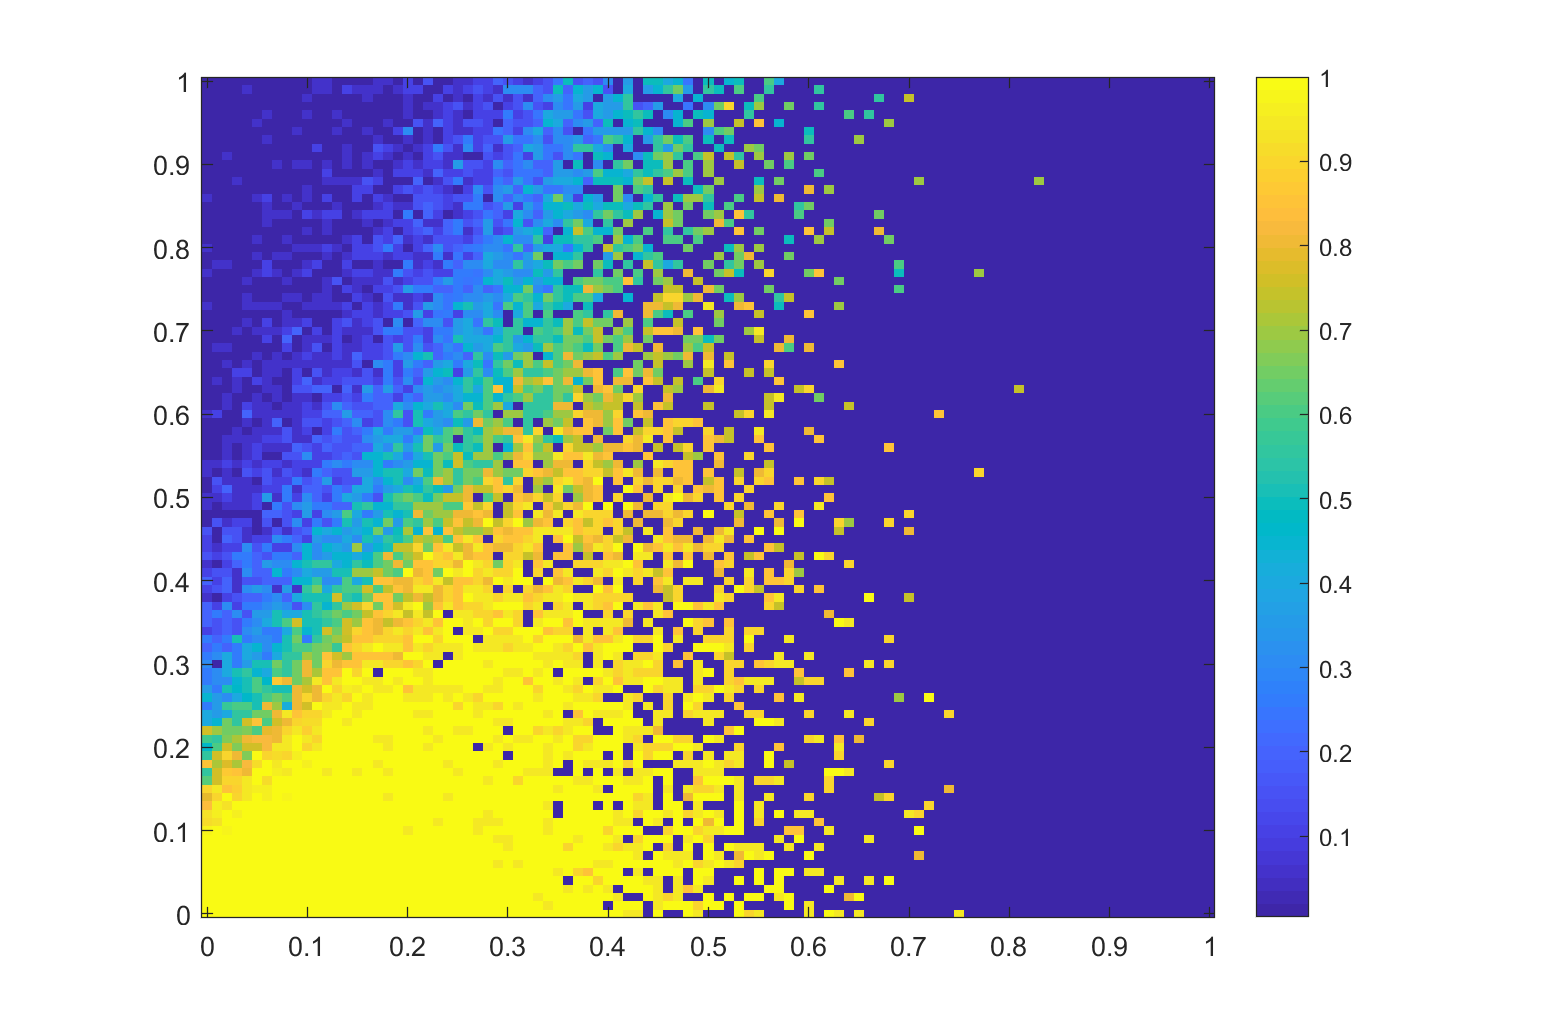
\includegraphics[scale=0.45]{FastAvgFixed.png}};
		\node[below] at (0, -5.5) {Death Rate $(\mu)$};
		\node[left, rotate=90] at (-8, 1) {Birth Rate $(\beta)$};
		\end{tikzpicture}
		
		\caption{Average value of $R_\infty^A$ for 50 simulations per parameter pair.}
		\label{fig:FastAvg}
		
	\end{figure}


	First, the uninteresting region is shaded blue (B cells survive) on the right side of the graph. This region is one with a very high death rate ($\mu > 0.5$) so eventually both populations go extinct. In this region, A cells tend to go extinct first, presumably because they cannot reproduce themselves, whereas B cells are able to reproduce, thus coloring the region blue.
	
	The two interesting regions are the roughly triangular regions on the left. The first of these areas (yellow region, lower left) tends to fairly robustly favor survival of A cells and the extinction of B cells. This corresponds to low birth rate and low death rate. The other region corresponds to low death rate, high birth rate and favors B cell survival.
	
	Our best chance at finding a non-trivial equilibrium state would be found along the boundary where these two regions meet. In fact, at first glance, we see that along this boundary $R_\infty^A \approx 0.6$, which could indicate a stable equilibrium of A and B cells together. However, we recall that this average is taken across 50 simulations and look at the variance of $R_\infty^A$ for these simulations in Figure \ref{fig:FastVar} to see that the this boundary region is also the region of highest variance. The conclusion to be drawn from this is that we do not, in fact, have a stable equilibrium where A and B cells exist alongside each other, but rather an unstable region where for any given simulation, we have an equal probability of tending towards an A extinction or a B extinction. Thus, we seem to have found conclusive evidence that we cannot find a region with a non-homogenous equilibrium state. 
	

	\begin{figure}[hbt]
		\centering
		\begin{tikzpicture}
		\node(img){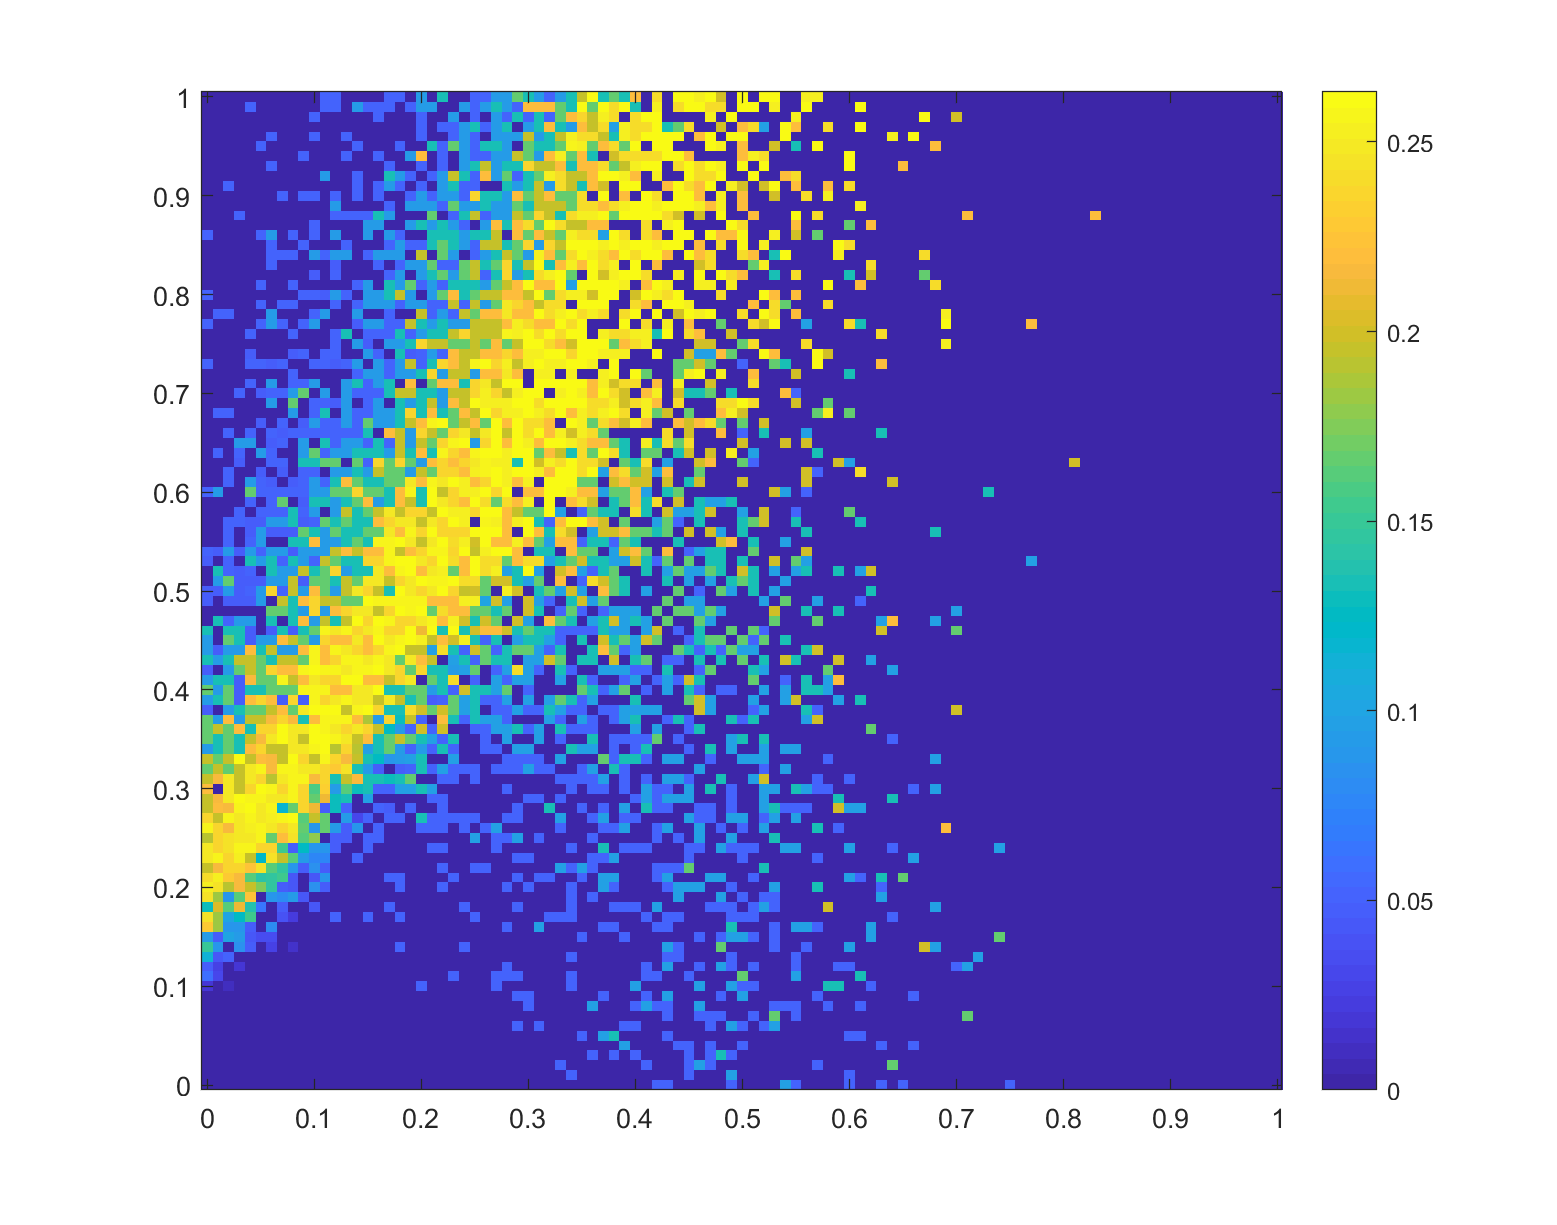
\includegraphics[scale=0.4]{FastVarFixed.png}};
		\node[below] at (0, -5.5) {Death Rate $(\mu)$};
		\node[left, rotate=90] at (-8, 1) {Birth Rate $(\beta)$};
		\end{tikzpicture}
		
		\caption{Variance of $R_\infty^A$ for 50 simulations per parameter pair.}
		\label{fig:FastVar}
		
	\end{figure}
	
	
	
	\newpage
	
	
	
	\part*{Project 2: Ising Model}
	
	
	\section*{Introduction}
	
	This project was a 2-D Ising model run on a $60\times 60$ grid with periodic boundary conditions. Each cell in the grid could take the values $\pm 1$ representing ON or OFF, respectively, i.e. if $c_{i,j}$ denotes the cell at position $(i,j)$, then $c_{i,j} \in \{1, -1\}$.	The model is run according to a Monte Carlo Method. That is, at each step a cell is chosen at random and ``flipped'' from ON to OFF, or vice versa. If this change results in a more favorable energy configuration, then the change is accepted, if not, it may still be accepted with some prescribed probability. More specifically, for a given energy function $E[\{s_i \}]$, define 
	\[\Delta E := E_{\text{new}} - E_{\text{old}}. \]
	Then the probability of a change being accepted is given by
	\[P(\text{flip}) = \min\left\{1, e^{-\Delta E} \right\}. \]
	
	\section*{Methods} 
	
	The backbone of this model is the energy function $E[\{s_i \}]$, so we discuss it here. This function is defined as follows:
	\[E[\{s_i \}] = -h \sum_i s_i - \frac{1}{2} \sum_{i, j} J(r_{i,j}) s_i s_j.  \]
	Here $h$ is a parameter that represents towards ON or OFF depending on its sign, $r_{i,j}$ is the distance between the $i$-th and $j$-th cells, and $J(r_{i,j})$ is a function dictating the interaction bewteen cells that depends on this distance. In our model, we took $J$ to be a step function, where for some cutoff radii $R_1 < R_2$, $J$ is constant within each radius and zero outside, in other words:
	\[J(r_{i,j}) = \begin{cases}
	J_1, & 0 < r_{i,j} \leq R_1\\
	J_2, & R_1 < r_{i,j} \leq R_2\\
	0, & R_2 < r_{i,j}.
	\end{cases} \]
	
	The simulation begins with a randomly chosen initial configuration. The simulation continues to run until there is very little energy change for a large number of iterations, currently set to 300 iterations. Note that the energy change will never be equal to zero, since unfavorable energy changes are accepted probabilistically. There is also a maximum run time of 100,000 iterations. These conditions together are almost always sufficient to view the resulting patterns.
	
	
	
	\section*{Results}	
	
	To view the results of these simulations, there are two options. First, to watch the simulation with a randomly chosen set of parameter values, one simply needs to run the file ``testRandomParameter.m.'' Running this file chooses the parameters randomly from a prescribed range, so successive runs of this file should produce vastly different results. The second option is to run the file ``runSavedParameter.m.'' This file contains saved parameter values that result in qualitatively different (and interesting!) patterns. To view the different saved patterns, one simply needs to comment/uncomment lines in the first section so that only one line of `params' is uncommented.
	
	Below are some examples of the wide range of patterns generated, along with the parameter values used.
	
	\begin{figure}[hbt]
		\centering
		\begin{tikzpicture}
		\node(img){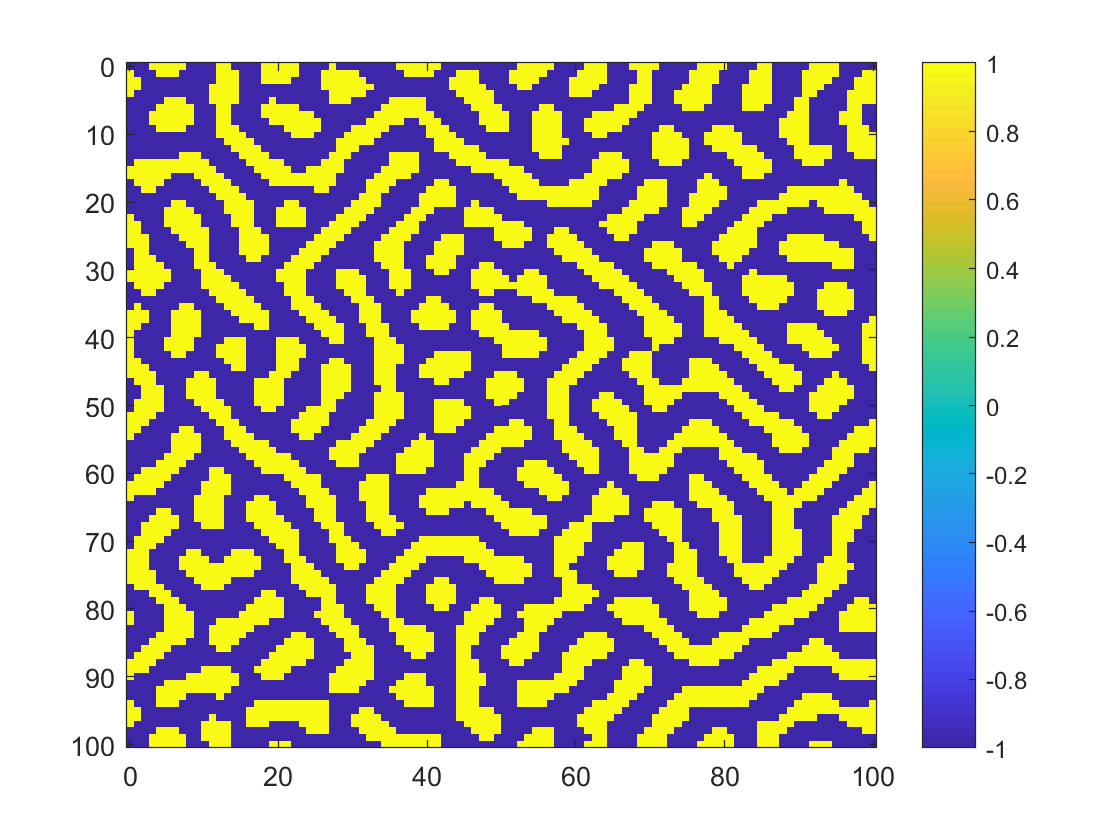
\includegraphics[scale=0.5]{SwirlyStripes.png}};
		\end{tikzpicture}
		
		\caption{$h = -2.73$, $R_1 = 1.91$, $J_1 = 1.73$, $R_2 = 5.30$,  $J_2 = -0.40$}
		\label{fig:FastVar}
		
	\end{figure}

	\begin{figure}[hbt]
		\centering
		\begin{tikzpicture}
		\node(img){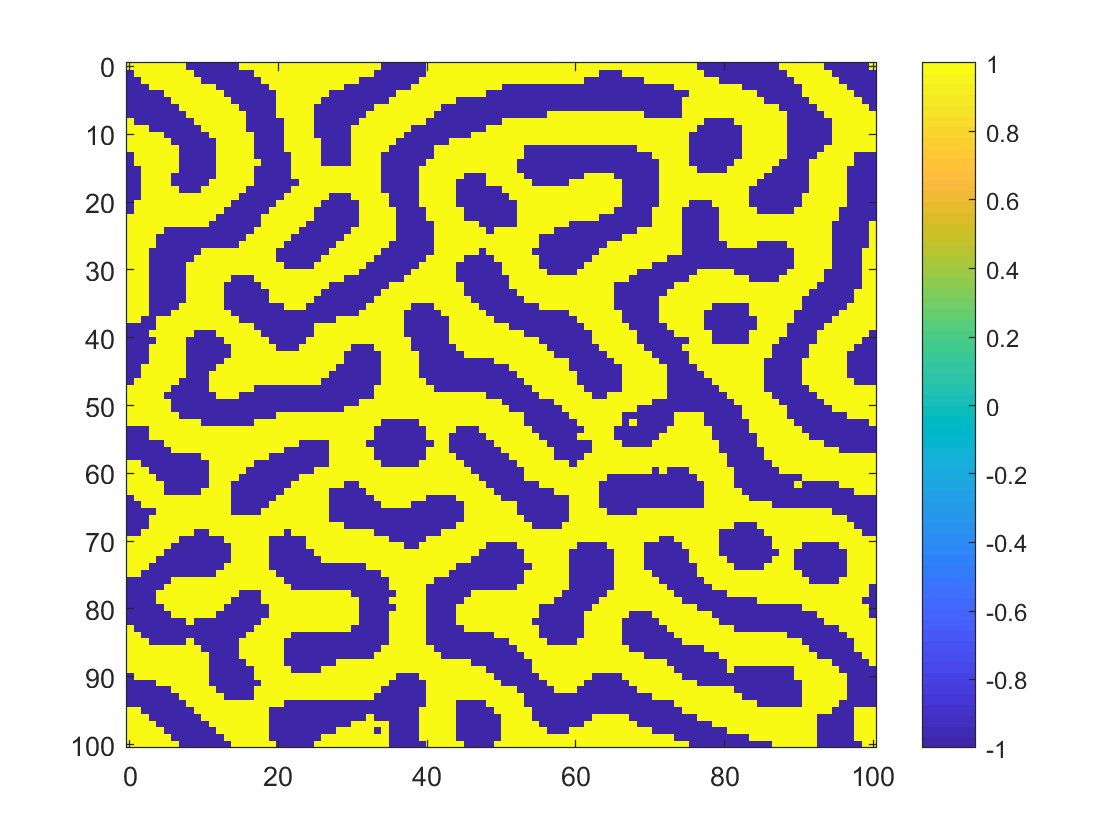
\includegraphics[scale=0.45]{ThickSwirls.png}};
		\end{tikzpicture}
		
		\caption{$h = 4.93$, $R_1 = 3.02$, $J_1 = 2.62$, $R_2 = 7.18$,  $J_2 = -0.82$}
		\label{fig:FastVar}
		
	\end{figure}

	\begin{figure}[hbt]
		\centering
		\begin{tikzpicture}
		\node(img){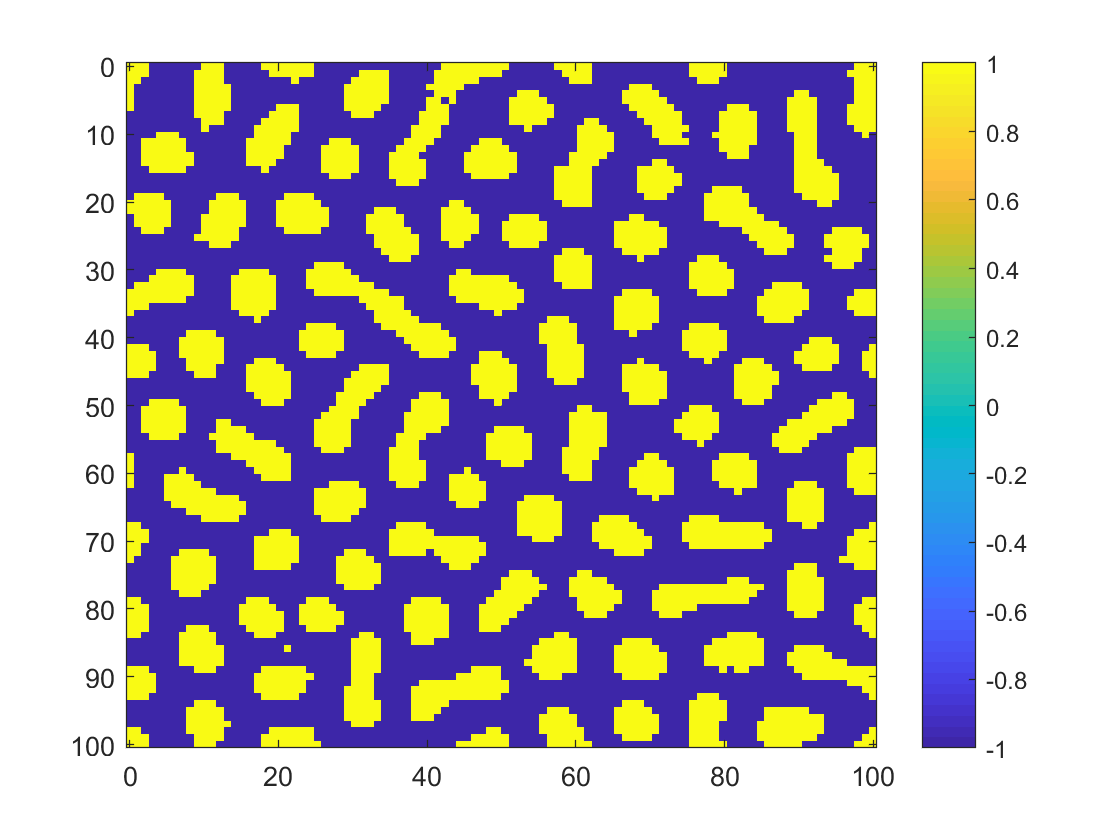
\includegraphics[scale=0.45]{LongSpots.png}};
		\end{tikzpicture}
		
		\caption{$h = -13.47$, $R_1 = 2.80$, $J_1 = 2.43$, $R_2 = 6.80$,  $J_2 = -0.73$}
		\label{fig:FastVar}
		
	\end{figure}


	\begin{figure}[hbt]
		\centering
		\begin{tikzpicture}
		\node(img){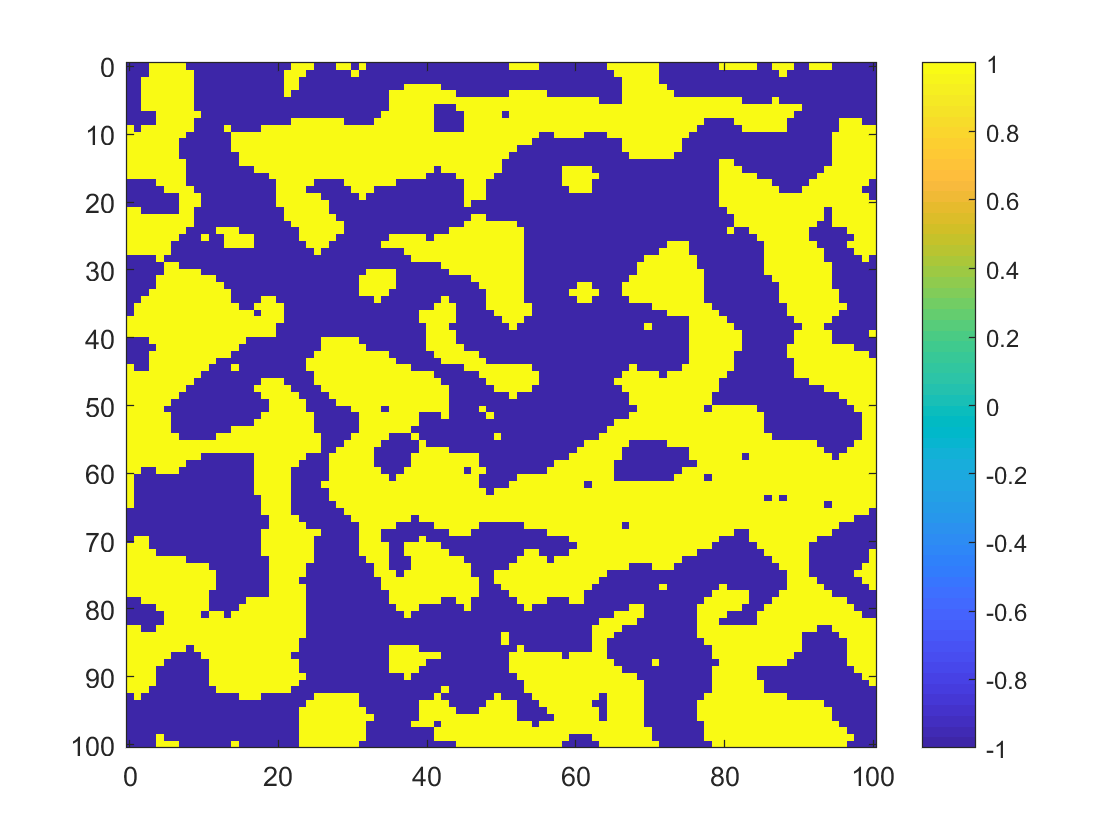
\includegraphics[scale=0.45]{OriginalIsingModel.png}};
		\end{tikzpicture}
		
		\caption{Original Ising Model with single radius: $h = 0$, $R_1 = 1.5$, $J_1 = 10$}
		\label{fig:FastVar}
		
	\end{figure}


	\begin{figure}[hbt]
		\centering
		\begin{tikzpicture}
		\node(img){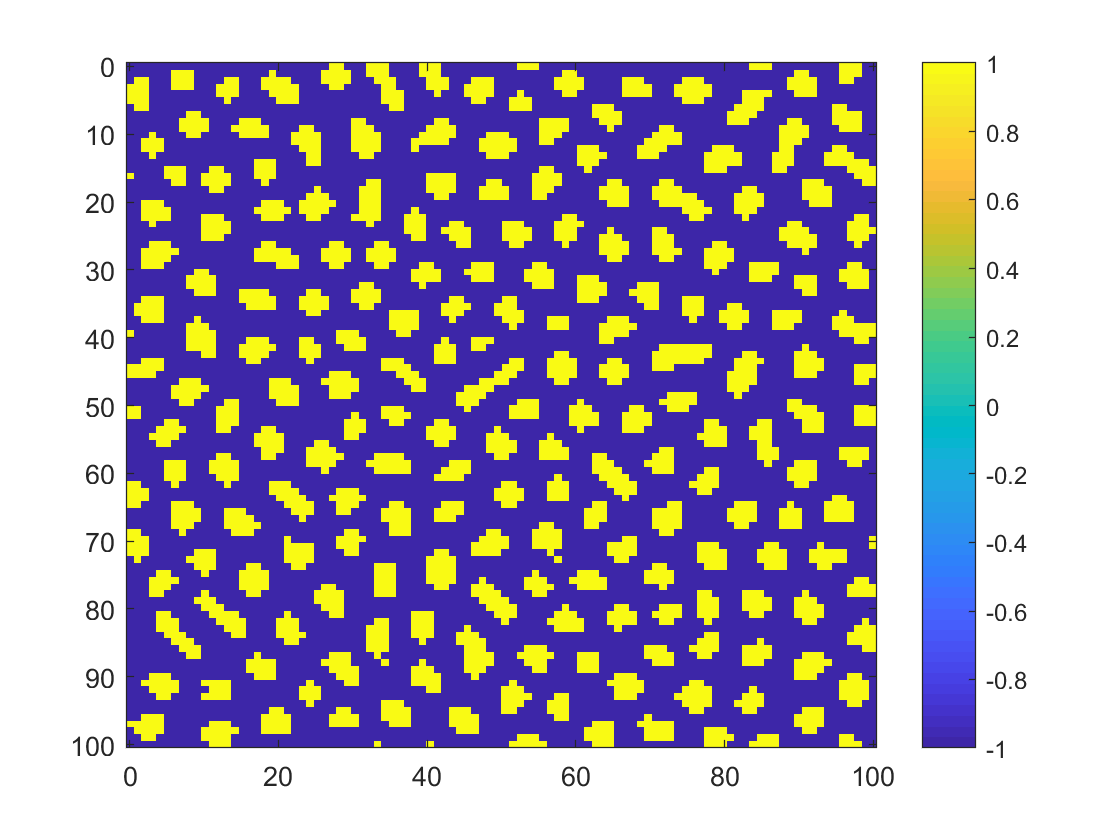
\includegraphics[scale=0.45]{SmallRegularSpots.png}};
		\end{tikzpicture}
		
		\caption{$h = -3.79$, $R_1 = 1.66$, $J_1 = 1.53$, $R_2 = 4.87$,  $J_2 = -0.30$}
		\label{fig:FastVar}
		
	\end{figure}
	
	
	
	
	
	\clearpage
	
	
	
	
	\part*{Summary Paper}
	\section*{A continuum approximation to an off-lattice individual-cell based model of cell migration and adhesion \cite{Middleton2014} }
	
	
	
%	\section*{Introduction}
%	
%	
%	
%	\section*{Summary}
%	
%	
%	
%	\section*{Results}	
%	
%	
%	
%	\section*{Conclusion}


	\section{Introduction}
	\indent 
	
	Cellular migration is of great interest to modelers due to the large range of situations it is necessary to take into account.  There have been a number of approaches to modeling this behavior, with the beginning models simplifying as much as possible.  Later models increase in sophistication as the previous models are shown to be either insufficient in capturing the behavior desired or are inscrutable from the perspective of using the model to extract connections between the model and the microscopic cell-scale processes.  The continuum approximation model proposed in this paper tries to address these two concerns first by identifying the deficiencies of previous pertinent models and then by extending those preceding models to compensate, resulting in a better continuum model.   
	
	
	\section{Previous Models Discussion}
	\indent
	
	The first model, a Mean Field Approximation, MFA, discussed revolves around a top-down approach, where a continuum-based model is derived from locally averaged properties such as spatial distributions of cell densities.  This approach relies on either well-established physical laws or by intuition to describe the motion of the cells, but assumes that the statistical correlation of cell-cell interactions are negligible.  Obviously this is problematic, as experimental data demonstrates clearly that there are strong interactions between cells and their nearby neighbors.  
	
	To try and capture this interaction between cells, IBM or "individual cell-based models," were created.  This model treats each cell as a discrete entity, whereas the previous continuum model treated them as an averaged value.  The first model using this discrete approach used a single node to describe the center of mass of each cell.  These nodes are then placed on a lattice grid, and the motion is simulated using transition probabilities.  These transition probabilities are where considerations such as volume exclusion and cell adhesion to either other cells or to the ECM are taken into account.  The probability of vacating a node is lowered if there are neighboring cells (adhesion), but the issue with this approach is that the coarseness of lattice.  The nodes representing the cells can be removed by more than the diameter of a cell, creating a non-lifelike condition that disallows the modelers from capturing correlations between the positions and velocities of the cells to each other.  Attacking this issue of coarseness, the next logical step is to create numerous nodes to describe a single cell.  A good example of this is the Cellular Potts Model.  This approach allows the model to capture the previously unavailable correlation data, but does so at the cost of computational time, as the lattice can be thought of as being refined into a finer mesh.  This computational cost induces investigation into off-lattice models.  These models are comparable to the on-lattice models in the sense that they too can either represent the cells as either centers of mass or a collection of nodes.  The difference is that off-lattice better captures the behaviors of the cells even in the coarsest settings where there are single nodes assigned to each cell, with the positions of these cells or subcellular cell elements being governed by either stochastics or ordinary differential equations.
	\section{Setup}
	
	\indent 
	
	The discrete model is the more accurate representation of the behavior of the cells, but comes at high computational cost.  Therefore, being able to connect the continuum models with the discrete model is ideal, as it would allow for the fast evaluation of variations of the parameter space.  A discrete model is introduced using an off-lattice IBM based on Langevin equations to begin this process of connection.  This model captures the adhesion and migration of the cells, and then is used to derive the governing equations for the associated probability distribution functions, which form a hierarchy of N partial integro-differential equations, where N denotes the number of cells in the system.  The discrete model is run multiple times, $10^5$ times to be exact, to create an "ensemble average" distribution, which creates numerical results by averaging the individual values across a large number of runs.  This ensemble average is compared against the results generated from two different continuum approximations, the MFA and the Kirkwood Superposition approximation, KSA.
	
	The continuum models are introduced as a strategy to try and truncate the hierarchy of integro-differential equations generated in the IBM model to a manageable amount.  This is achieved by comparing the results generated from the IBM against those of the continuum models to see if there is sufficient connection to justify using the continuum models as a tool for rapid investigation of the parameter space.  
	
	\section{IBM Construction and Discussion}
	
	\indent 
	
	The IBM used to capture cell movement and adhesion follows the model developed by Newman and Grima: 
	\[\dot{x_i} = \xi_i + \alpha \nabla_i \phi.\]  
	
	The $\xi$ term encompasses noise, $\alpha$ represents the chemotactic attitude, with positive indicating aggregation and negative, repulsion. The gradient of $\phi$, the chemical concentration, is evaluated at the cell's current position.  The IBM model assumes that the cells are point masses, and is constructed using Newton's second law, 
	\[m_i \frac{d^{2}x_{i}}{dt^2}=F^{visc}_i+\sum_{k,k\neq i}F^{int}_{i,k}+\xi_i.\]
	
	Here, $m_i$ represents the mass of cell i, $x_i$ the position, $F^{int}_{i,k}$ the force generated by the interactions between cells i and k, $F^{visc}_i$ the viscous force acting on cell i, and $\xi_i$ the stochastic force representing self-propulsion.  The $\xi$ values that are used in this model are sampled from a Gaussian distribution with zero mean and zero auto-correlation as follows:
	\[
	<\xi_i(t),\xi_j(t')>=2D\delta_{i,j}\delta(t-t').
	\] 
	Note that the D in the Gaussian distribution represents the constant of proportionality, which corresponds to the cell diffusion coefficient.  This allows for the assumption that cells will move randomly when isolated, but will experience mechanical interactions with their neighbors if they are proximally relevant.  Additionally, the viscous substrate acting on cell i with a drag force can be assumed to be proportional to the cell's velocity, with value $\mu$, which can thus be ignored.  This is acceptable because there is a low Reynolds number at the scale of the cellular length, which implies that the inertial forces $F^{visc}$ can be neglected.  There are further assumptions that the interaction forces can be written as 
	\[
	F^{int}_{i,k}=\hat{F}_0 F \left( \lVert x_i -x_j \rVert \right) \frac{x_i -x_j}{\lVert x_i -x_j \rVert}.
	\]
	Here, F is a scalar function of the separation between pairs of cells, and $\hat{F}_0$ contains the dimensional proportionality constant that captures the various mechanical forces.  This term is particularly important as this term includes the cell-cell adhesion and cell resistance to deformation.  This leads to the final equation
	\[
	\frac{dx_i}{dt}=F_0 \sum_{k,k\neq i} F \left( \lVert x_i -x_j \rVert \right) \frac{x_i -x_j}{\lVert x_i -x_j \rVert} + \xi_i,
	\]
	where $F_0 =\hat{F_0}/\mu$.  For the sake of accuracy, non-linear force laws based on phenomenological principles is adopted, namely the Morse Potential, to describe $F$, as
	\[
	F(r)=\left\lbrace \begin{array}{ll}	2(exp(-2a(r-r_c))-exp(-a(r-r_c)), &r<\sigma r_c\\
	0, & r\geq \sigma r_c \end{array}\right.
	\]
	$F(r)$ contains both attraction representing cell-cell adhesion, ($r>r_c$), and repulsion representing resistance to cellular deformation, ($r\geq r_c$).  The mechanical interactions between the cell is restricted by $\sigma r_c$, where $\sigma$ is the distance at which cells may interact, given in terms of multiples of cell-radii.  The longer range interactions, biologically relevant due to motility protrusions such as filopodia, may be ignored as the protrusions are typically on the length scale of one cell radius, which falls below the $\sigma$ threshold.  The range that is considered for this model is $1<\sigma\leq 3$, where $\sigma \leq 1$ generates repulsive forces only.
	
	Additional considerations include the nondimensionalization of length and time as follows: \[x^{*}=\frac{x}{L},\\
	t^{*}=\frac{t}{L^2/D}.\] 
	Therefore the final equations which govern motion for this model are 
	\[
	\frac{dx^{*}_i}{dt}=F^{*}_0 \sum_{k,k\neq i} F \left( \lVert x^{*}_i -x^{*}_j \rVert \right) \frac{x^{*}_i -x^{*}_j}{\lVert x^{*}_i -x^{*}_j \rVert} + \xi^{*}_i\]
	\[
	<\xi^{*}_i(t),\xi^{*}_j(t')>=2D\delta_{i,j}\delta(t^{*}-t^{*'})
	\] 
	and
	\[
	F^{*}(r)=\lbrace \begin{array}{ll}	2(exp(-2a^{*}(r^{*}-\epsilon)/\epsilon)-exp(-a^{*}(r^{*}-\epsilon)/ \epsilon))/\epsilon, &r<\sigma r_c\\
	0, & r\geq \sigma r_c,
	\end{array}
	\]
	with
	\[
	F^{*}(r^{*})=\frac{F_0 L}{D}, \epsilon=\frac{r_c}{L}, a^{*}=a r_c.
	\]  In actuality, the term $\epsilon$ is considered to be extremely small, and thus the superscripts are dropped and work is done exclusively with the dimensionless model.
	
	\section{One and two-cell probability density functions}
	\indent
	
	The dimensionless IBM can now be represented using probability density functions, PDF.  There is an assumption that the boundary is periodic, The one-cell PDF is defined as 
	\[
	P_i(\textbf{x},t) = \langle \delta ( x - x_i(t))\rangle,
	\]
	the two-cell PDF as 
	\[
	P_i(\textbf{x},\textbf{x'},t) = \langle \delta ( x - x_i(t))\delta ( x' - x_j(t))\rangle,
	\] and thus with manipulation, we obtain 
	\[
	\frac{\partial P_i(x,t)}{\partial t} = - \nabla^2 P_i -F_0\nabla \int F \left( \lVert x -x' \rVert \right) \frac{x-x'}{\lVert x-x' \rVert}p_2(x,x',t)dx'
	\] and the therefore the final governing equations
	\[
	\frac{\partial p_1(x,t)}{\partial t} = \nabla^2 p_1(x,t)-F_0(N-1)\nabla \int F \left( \lVert x_i -x_j \rVert \right) \frac{x-x'}{\lVert x-x' \rVert}p_2(x,x',t)dx'
	\]
	\[
	\begin{array}{lll}
	\frac{\partial p_2(x,x',t)}{\partial t}&=&\nabla^2 p_2(x,x',t)-F_0(\frac{\partial}{\partial x}-\frac{\partial}{\partial x'})\times\left(F \left( \lVert x -x' \rVert \right) \frac{x-x'}{\lVert x-x' \rVert}p_2(x,x',t)\right)\\
	&&-F_0(N-2)\frac{\partial}{\partial x}\int F \left( \lVert x -x'' \rVert \right) \frac{x -x''}{\lVert x -x'' \rVert}p_3(x,x',x'',t)dx''\\
	&&-F_0(N-2)\frac{\partial}{\partial x'}\int F \left( \lVert x' -x'' \rVert \right) \frac{x' -x''}{\lVert x' -x'' \rVert}p_3(x,x',x'',t)dx''.\\
	\end{array}
	\]
	\section{The Mean Field Approximation, "MFA"}
	\indent
	
	
	The number of equations necessary to properly model the behavior of N cells requires N integro-differential equations, which is computationally undesirable.  In adapting a closure method, the number of equations can be truncated to a more tractable problem.  Truncating at the first level corresponds to writing down the density-density correlation function in terms of the cell density distribution.  Precisely this means that
	\[
	p_2(x,x',t)=p_1(x,t)p_1(x',t).
	\]
	Therefore 
	\[
	\frac{\partial p_1(x,t)}{\partial t} = - \nabla^2 p_1(x,t) -F_0(N-1)\nabla \cdot (p_1(x,t)\phi(x,t),
	\]
	with
	\[
	\phi(x,t)=\int F \left( \lVert x -x' \rVert \right) \frac{x -x'}{\lVert x -x' \rVert}p_1(x',t)dx'.
	\]
	\section{The Kirkwood superposition approximation, "KSA"}
	\indent
	
	The MFA appears to not provide adequate approximations to the cell-density distribution generated through the ensemble approximation given by the IBM model.  This induces the development of an alternative closure relation, the Kirkwood Superposition Approximation.  This takes the form of 
	\[
	p_3(x,x',x'',t)=\frac{p_2(x,x',t)p_2(x,x'',t)p_2(x',x'',t)}{p1(x,t)p1(x',t)p1(x'',t)},
	\]
	which is typically a good approximation in the limits of low densities and is a valuable tool to approximate off-lattice models of cells.  The explicit formula for the KSA, analogous to the first governing equation of our IBM model is 
	\[
	\begin{array}{lll}
	\frac{\partial p_2(x,x',t)}{\partial t}&=&\nabla^2 p_2(x,x',t)-F_0(\frac{\partial}{\partial x}-\frac{\partial}{\partial x'})\\
	&&\times\left(F \left( \lVert x -x' \rVert \right) \frac{x-x'}{\lVert x-x' \rVert}p_2(x,x',t)\right)-F_0(N-2)\frac{\partial}{\partial x}\\
	&&\times \int F \left( \lVert x -x'' \rVert \right) \frac{p_2(x,x',t)p_2(x,x'',t)p_2(x',x'',t)}{p1(x,t)p1(x',t)p1(x'',t)}dx''\\
	&&-F_0(N-2)(\frac{\partial}{\partial x'}\int F \left( \lVert x' -x'' \rVert \right)\times \frac{x'-x''}{\lVert x' -x'' \rVert}\frac{p_2(x,x',t)p_2(x,x'',t)p_2(x',x'',t)}{p1(x,t)p1(x',t)p1(x'',t)}dx''
	\end{array}
	\]
	\section{Numerical Methods and Discussion}
	\indent 
	
	
	For the purposes of comparison, the models are all restricted to one dimension.  The comparisons are made between the estimates of cell-density and density-density correlation functions that are obtained from the IBM and those obtained from the MFA and KSA.  As both the MFA and KSA models take the form of advection-diffusion, particularly the KSA, there is a consideration taken for the peaks that can naturally form in the density-density correlation functions in the $x-x'$.  Therefore it becomes expedient to rewrite the equations for the using the center of mass $\eta=x+x'$ and $\xi=x-x'$, where 
	\[
	\eta =  \left\lbrace \begin{array}{lll}
	\xi&for& 0<\eta\leq 1,\\
	2-\xi&for&1<\eta\leq 2.
	\end{array} \right. \]
	
	The MFA and KSA models were both run by first discretising the space, and then integrating the ODEs.  This was compared with the IBM, where the Euler-Maruyama method is employed, with timesteps of size $\Delta t=10^{-7}$ and $t\in [0,10^{-2}]$.  There were 51 points taken from this model, at regular intervals. 
	
	The initial conditions for the IBM model are as follows:
	\[
	p_0(x)=\frac{f(x)}{\int_0^1 f(x)dx}
	\]
	and 
	\[
	f(x)=\frac{1}{2}(tanh(\alpha(x-\theta))+tanh(\alpha(1-\theta-x))),
	\]
	with $\theta=0.2$ and $\alpha=30$ for all simulations.  These conditions correspond to cells being densely packed in a one-dimensional environment.  These results are compared to the density-density correlation function of the MFA and KSA by computing 
	\[
	E=\frac{1}{MT}\sum\limits_{i,j}(p_1(i,j)-p^{ens}_1(i,j))^2. 
	\]   Setting $1\leq i\leq M$ and $1\leq j \leq T$, where T=51, the results depend on the beginning parameters, and thus the paper provides examples of the numerical results with different beginning parameters in graphical form to help a reader visualize the difference in variability.
	
	Comparisons between the results of the IBM run $10^5$ times against either the MFA or the KSA results in the understanding that the KSA model is superior to the MFA as a continuum approximation.  The primary driving force for this conclusion results from the fact that the KSA develops the same peaks in the density-density correlation that are induced in the IBM, while the MFA is constantly  disagreement.  The problems with the KSA arise when intercellular forces are weak, and so the $F_0$ is increased to make each of the peaks sharp compared to the results generated by the IBM.  The differences between the MFA and the KSA are most easily found demonstrated by varying the sensing ranges ($\sigma$), the intercellular force strength ($F_0$), and relative densities $\rho$.  The KSA is going to be much more robust in terms of being able to properly describe cell-cell interactions when there are both weak interacting cells and when there are high densities to consider.  This is contrasted by the MFA, which is most useful when $F_0$ is low.  This same idea holds true with other parameter variations as well, indicating that the KSA is a preferable method for continuum approximation.
	\section{Summary}
	\indent
	
	The KSA model is identified as being a much more relevant continuum approximation to the IBM models.  This model is able to capture behaviors simulated in the IBM under a variety of conditions, exceeding the ability of the MFA to handle both low and high densities.  Additionally, the KSA is able to incorporate other cell-level phenomena such as heptotaxis.  The issues of the model arise when there are few cells that are motile (cancerous metastasis for example).  Additionally, the computational challenges of validating the KSA model against the IBM model in higher dimensions requires a more refined approach to the numerical approximations of the KSA model.  The computational requirements are going to be prohibitive as there are formulas arising from each dimension.  Thus, the next step of research along these particular lines involves looking into the Johnson-Kendall-Roberts model, that incorporates adhesive elastic spheres. The most obvious area for improvement stems from the fact that the models all are supposing that the cells are represented by center of mass nodes.  The KSA model is good to approximate the results of the IBM for both small and large cell population sizes, cell propulsion and mechanical forces.  This is wonderful, as it allows the modeler to evaluate parameter variation without endeavoring to run $10^5$ simulations on the IBM!

	
	\printbibliography
	
	
	
\end{document}
